\documentclass{article}

\usepackage[final]{style}
\usepackage[utf8]{inputenc} % allow utf-8 input
\usepackage[T1]{fontenc}    % use 8-bit T1 fonts
\usepackage{hyperref}       % hyperlinks
\usepackage{url}            % simple URL typesetting
\usepackage{booktabs}       % professional-quality tables
\usepackage{amsfonts}       % blackboard math symbols
\usepackage{nicefrac}       % compact symbols for 1/2, etc.
\usepackage{microtype}      % microtypography
\usepackage{verbatim}
\usepackage{graphicx}       % for figures
\usepackage{placeins}
\usepackage{amsmath}
\usepackage{gensymb}

\title{Lecture \#06: Edge Detection}

\author{
  Winston Wang, Antonio Tan-Torres, Hesam Hamledari \\
  Department of Computer Science\\
  Stanford University\\
  Stanford, CA 94305 \\
  \texttt{\{wwang13, tantonio\}@cs.stanford.edu; hesamh@stanford.edu} \\
}

\begin{document}
\maketitle
\section{Introduction}
This lecture covers edge detection, Hough transformations, and RANSAC.
The detection of edges provides meaningful semantic information that facilitate the understanding of an image. This can help analyzing the shape of elements, extracting image features, and understanding changes in the properties of depicted scenes such as discontinuity in depth, type of material, and illumination, to name a few. We will explore the application of Sobel and Canny edge detection techniques.
The next section introduces the Hough transform, used for the detection of parametric models in images;for example, the detection of linear lines, defined by two parameters, is made possible by the Hough transform. Furthermore, this technique can be generalized to detect other shapes (e.g., circles).
However, as we will see, the use of Hough transform is not effective in fitting models with a high number of parameters. To address this model fitting problem, the random sampling consensus (RANSAC) is introduced in the last section; this non-deterministic approach repeatedly samples subsets of data, uses them to fit the model, and classifies the remaining data points as "inliers" or "outliers" depending on how well they can be explained by the fitted model (i.e., their proximity to the model). The result is used for a final selection of data points used in achieving the final model fit. A general comparison of RANSAC and Hough transform is also provided in the last section.

\section{Edge Detection}
\subsection{Motivation for Edge Detection}
Edge detection is extremely relevant for mammalian eyes.  Certain neurons within the brain are adept at recognizing straight lines.  The information from these neurons is put together in the brain for recognition of objects.  In fact, edges are so useful for recognition in humans, line drawings are almost as recognizable as the original image (Fig. 1).We would like to be able to extract information, recognize objects, and recover the geometry and viewpoint of an image.

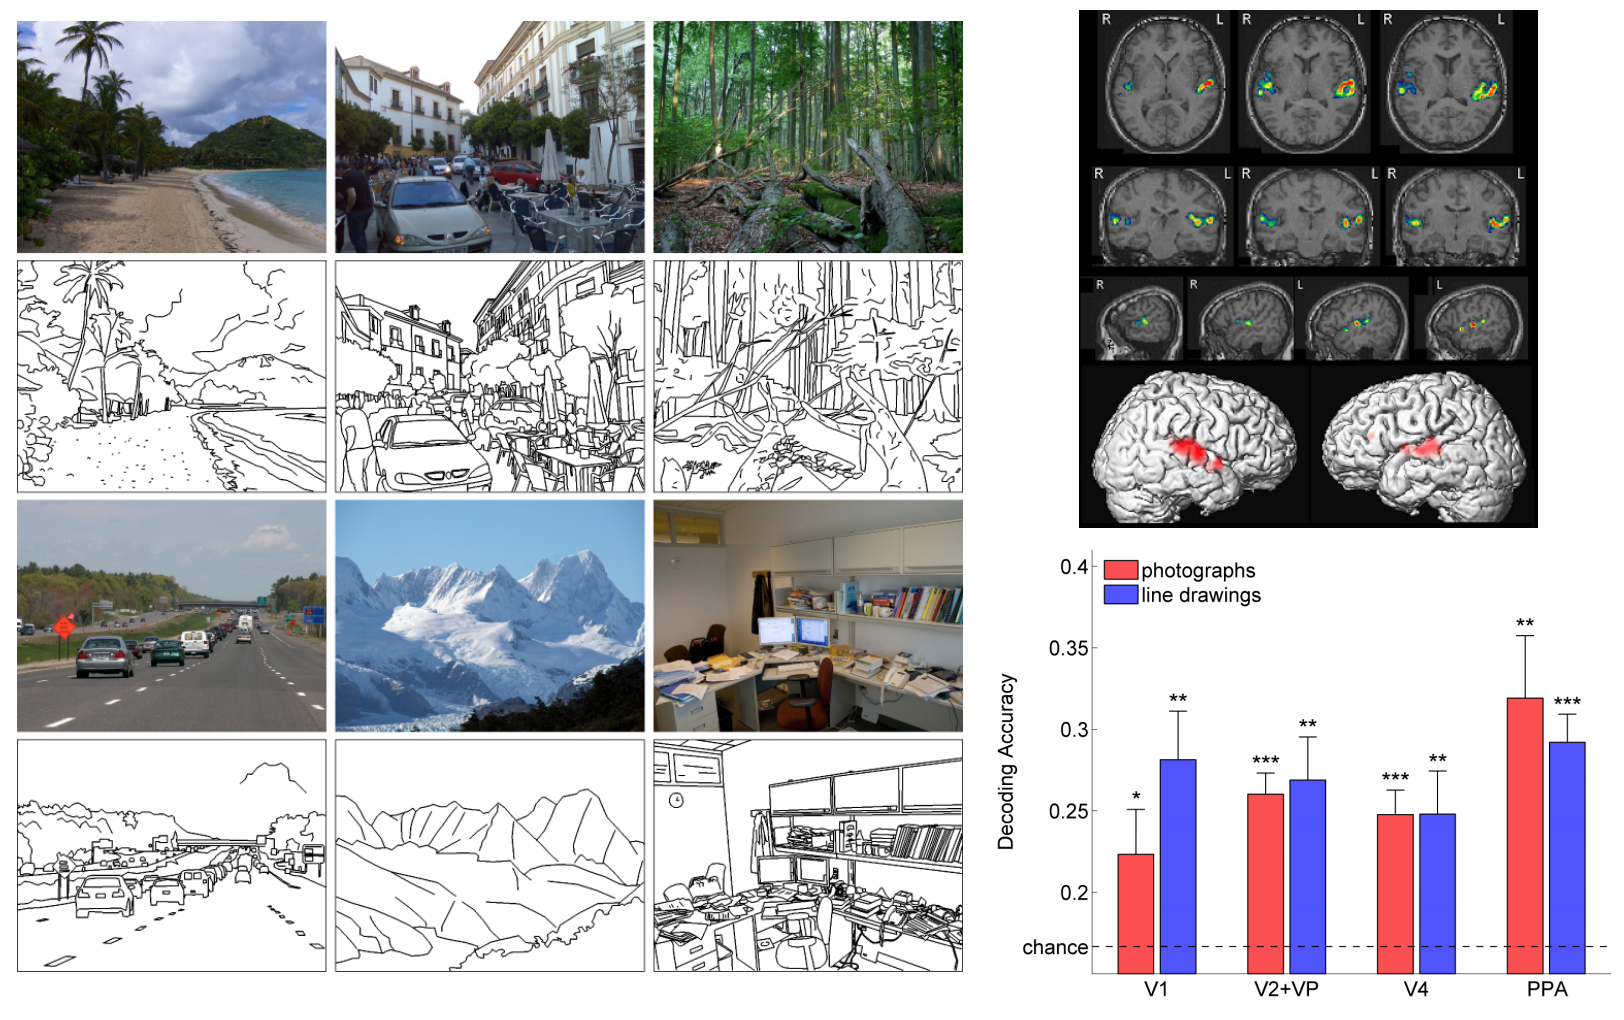
\includegraphics[width=\textwidth]{line_drawings.png}
\textbf{Fig. 1. Certain areas of the brain react to edges; the line drawings are as recognizable as the original image; image source: \cite{line_drawings}}

\subsection{Edge Basics}
There are four possible sources of edges in an image:  surface normal discontinuity (surface changes direction sharply), depth discontinuity (one surface behind another), surface color discontinuity (single surface changes color), illumination discontinuity (shadows/lighting).  These discontinuities are demonstrated in the Fig.2a; different types of edges can be seen in Fig.2b:
\FloatBarrier
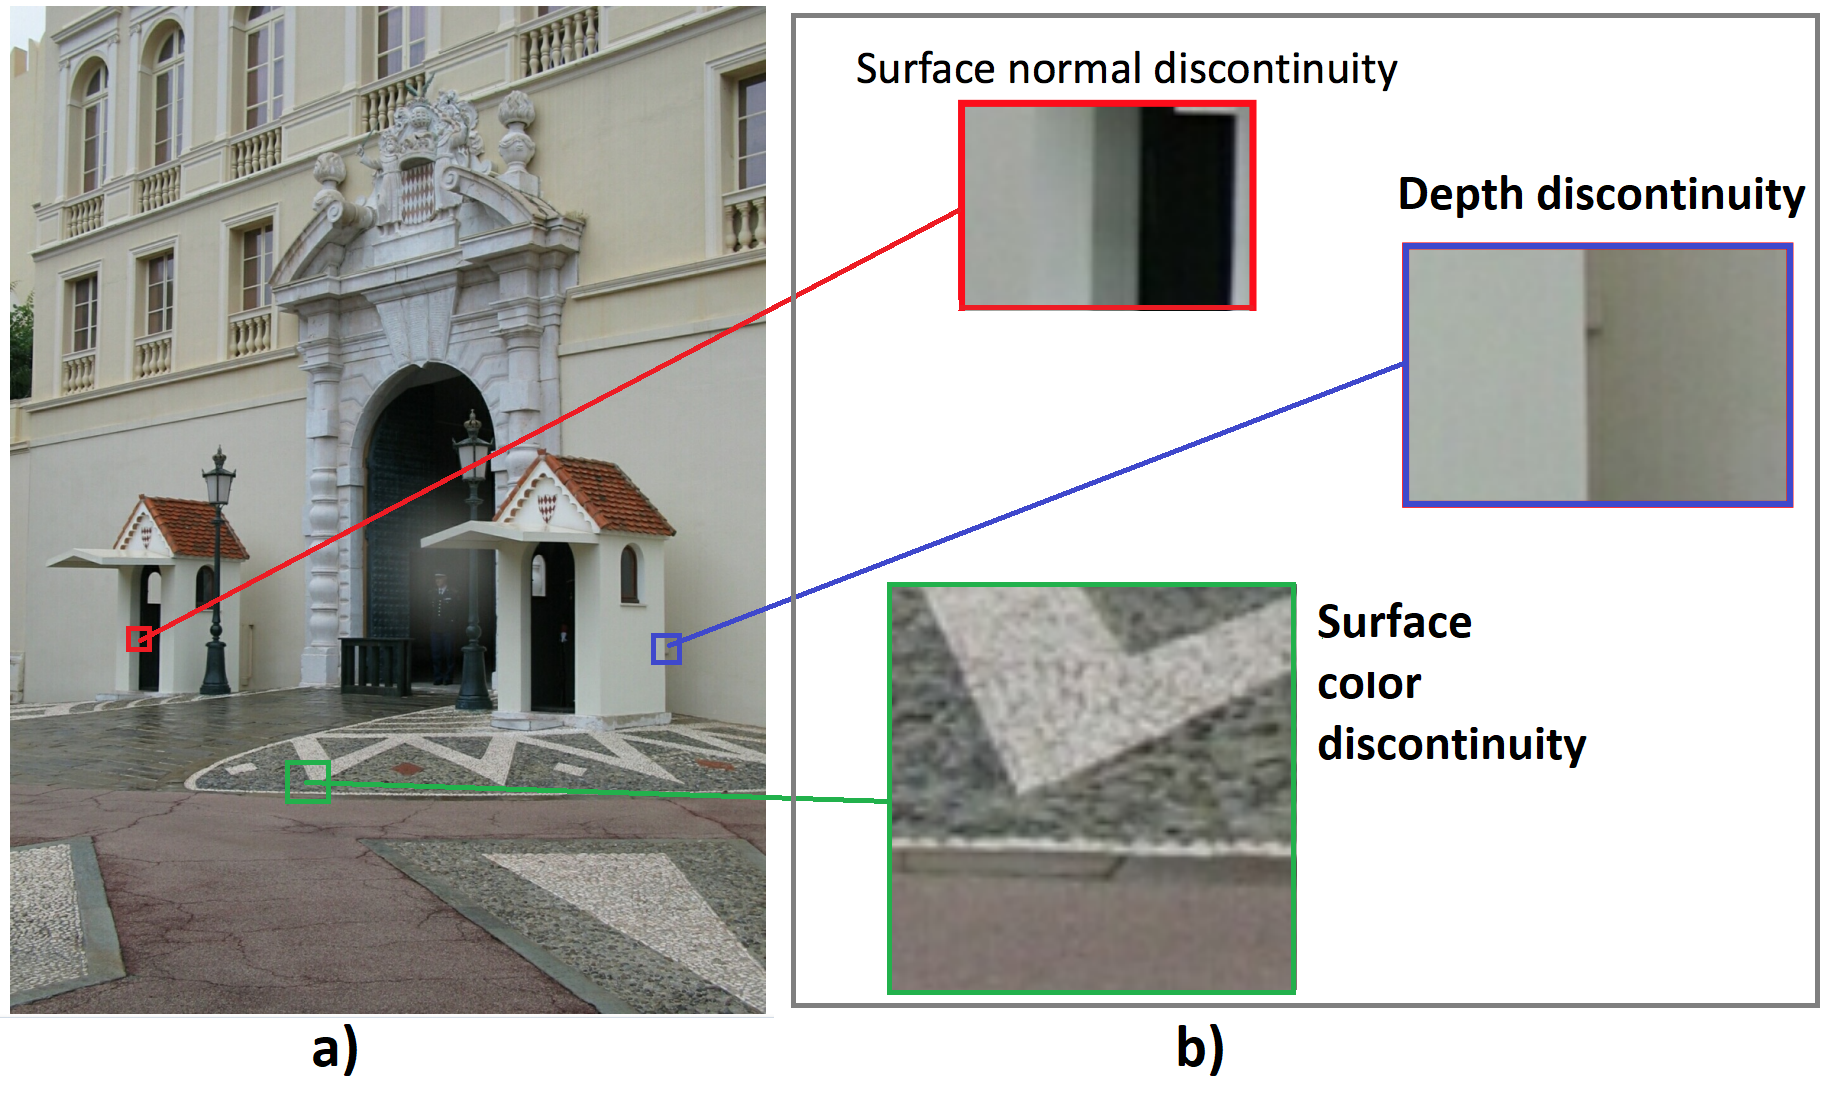
\includegraphics[width=\textwidth]{overall.png}
\FloatBarrier
\textbf{Fig. 2. Different types of edges due to discontinuities in surface color, surface depth, and surface normal (source: lecture notes)}

Edges occur in images when the magnitude of the gradient is high
\subsection{Finding the Gradient}
In order to find the gradient, we must first find the derivatives in both the $x$ and $y$ directions
\subsubsection{Discrete Derivatives}
\begin{align*}
\frac{df(x)}{dx} &= \lim_{\delta x\rightarrow0}\frac{f(x)-f(x-\delta x)}{\delta x} = f'(x)\\
\frac{df(x)}{dx} &= \frac{f(x)-f(x-1}{1} = f'(x)\\
\frac{df(x)}{dx} &= f(x)-f(x-1) = f'(x)
\end{align*}
It is also possible to take the derivative three different ways
\begin{itemize}
\item Backward: $f'(x) = f(x)-f(x-1)$
\item Forward: $f'(x) = f(x+1)-f(x)$
\item Central: $f'(x) = \frac{(x+1)-f(x-1)}{2}$
\end{itemize}
Each of these can also be represented as a filter (convoluting the filter with the image gives the derivative)
\begin{itemize}
\item Backward: $f'(x) = f(x)-f(x-1)\rightarrow[0,1,-1]$
\item Forward: $f'(x) = f(x)-f(x+1)\rightarrow[-1,1,0]$
\item Central: $f'(x) = f(x+1)-f(x-1)\rightarrow[1,0,-1]$
\end{itemize}
The gradient ($\nabla f$) can be calculated as follows:
\begin{align*}
\nabla f(x,y) &= \begin{bmatrix}%
    \frac{\partial f(x,y)}{\partial x}\\
    \frac{\partial f(x,y)}{\partial y}
    \end{bmatrix}\\
    &= \begin{bmatrix}%
    f_x\\
    f_y
    \end{bmatrix}
\end{align*}
We can also calculate the magnitude and the angle of the gradient:
\begin{align*}
|\nabla f(x,y)| &= \sqrt{f_x^2+f_y^2}\\
\theta &= \tan^{-1}\left(f_y/f_x\right)
\end{align*}
\subsection{Reducing noise}
Noise will interfere with the gradient, making it impossible to find edges using the simple method, even though the edges are still detectable to the eye.  The solution is to first smooth the image.
\newline
Let $f$ be the image and $g$ be the smoothing kernel.  Thus, in order to find the smoothed gradient, we must calculate (1D example):
\[
\frac{d}{dx}(f*g)
\]
By the derivative theorem of convolution:
\[
\frac{d}{dx}(f*g) = f*\frac{d}{dx}g
\]
This simplification saves us one operation.  Smoothing removes noise but blurs edges.  Smoothing with different kernel sizes can detect edges at different scales
\subsection{Sobel Noise Detector}
This algorithm utilizes 2 $3\times3$ kernels which, once convolved with the image, approximate the $x$ and $y$ derivatives of the original image.
\begin{align*}
&\mathbf{G}_x = \begin{bmatrix}%
    1 & 0 & -1\\
    2 & 0 & -2\\
    1 & 0 & -1
    \end{bmatrix}
    &\mathbf{G}_y = \begin{bmatrix}%
    1 & 2 & 1\\
    0 & 0 & 0\\
    -1 & -2 & -1
    \end{bmatrix}
\end{align*}
These matrices represent the result of smoothing and differentiation
\[
\mathbf{G}_x = \begin{bmatrix}%
    1 & 0 & -1\\
    2 & 0 & -2\\
    1 & 0 & -1
    \end{bmatrix} = \begin{bmatrix}%
    1\\
    2\\
    1
    \end{bmatrix}\begin{bmatrix}%
    1 & 0 & -1\\
    \end{bmatrix}
\]
The Sobel Filter has many problems, including poor localization.  The Sobel Filter also favors horizontal and vertical edges over oblique edges
\subsection{Canny Edge Detector}
The Canny Edge Detector has five algorithmic steps:
\begin{itemize}
\item Suppress noise
\item Compute gradient magnitude and direction
\item Apply non-maximum suppression
\item Hysteresis thresholding
\item Connectivity analysis to detect edges
\end{itemize}
\subsubsection{Suppress noise}
We can both suppress noise and compute the derivatives in the $x$ and $y$ directions using a method similar to the Sobel filter.
\subsubsection{Compute gradient magnitude and direction}
From above,
\begin{align*}
|\nabla f(x,y)| &= \sqrt{f_x^2+f_y^2}\\
\theta &= \tan^{-1}\left(f_y/f_x\right)
\end{align*}
\subsubsection{Apply non-maximum suppression}
The purpose of this portion of the algorithm is to make sure the edges are specific.  Thus, we assume that the edge occurs when the gradient reaches a maximum.  We suppress any pixels that have a non-maximum gradient.\newline
Basically, if the pixel is not the largest of the three pixels in the direction and opposite the direction of its gradient, it is set to 0.  Furthermore, all gradients are rounded to the nearest 45\degree
\subsubsection{Hysteresis thresholding}
All remaining pixels are subjected to hysteresis thresholding.  This part uses two values, for the high and low thresholds.  Every pixel with a value above the high threshold is marked as a strong edge.  Every pixel below the low threshold is set to 0.  Every pixel between the two thresholds is marked as a weak edge
\subsubsection{Connectivity analysis to detect edges}
The final step is connecting the edges.  All strong edge pixels are edges.  For weak edge pixels, only the weak edge pixels that are linked to strong edge pixels are edges.  The part uses BFS or DFS to find all the edges.

\section{Hough Transforms}
\subsection{Intro to Hough Transform}
Hough Transform is a way to detect particular structures in images, namely lines. However, Hough transform can be used to detect any structure whose paramteric equation is known. It gives a robust detector under noise and partial occlusion.

\subsection{Goal of Hough Transform for detecting lines}
Hough transform can be used to detect lines in images. To do this, we want to locate sets of pixels that make up straight lines in the image. This works to detect lines in an image after an edge detector is applied to get the pixels of just the edges (and thus we find which sets of those pixels make up straight lines).

\subsection{Detecting lines using Hough Transform in a,b space}
Say we have a ${x_i,y_i}$. There are infinite lines that could pass through this point.
We can define a line that passes through this pixel $x_i, y_i$ as $$y_i = a*x_i + b$$. Using this, we can transform each pixel into $a,b$ space by re-writing this equation as:
$$ b = -a*x_i + y_i$$

This equation represents a line in $a,b$ space, and each $a,b$ point on the line represents a possible line passing through our point $x_i,y_i$.

Thus, for each pixel $x_i,y_i$ in our set of edge pixels, we transform it into $a,b$ space to get a line.

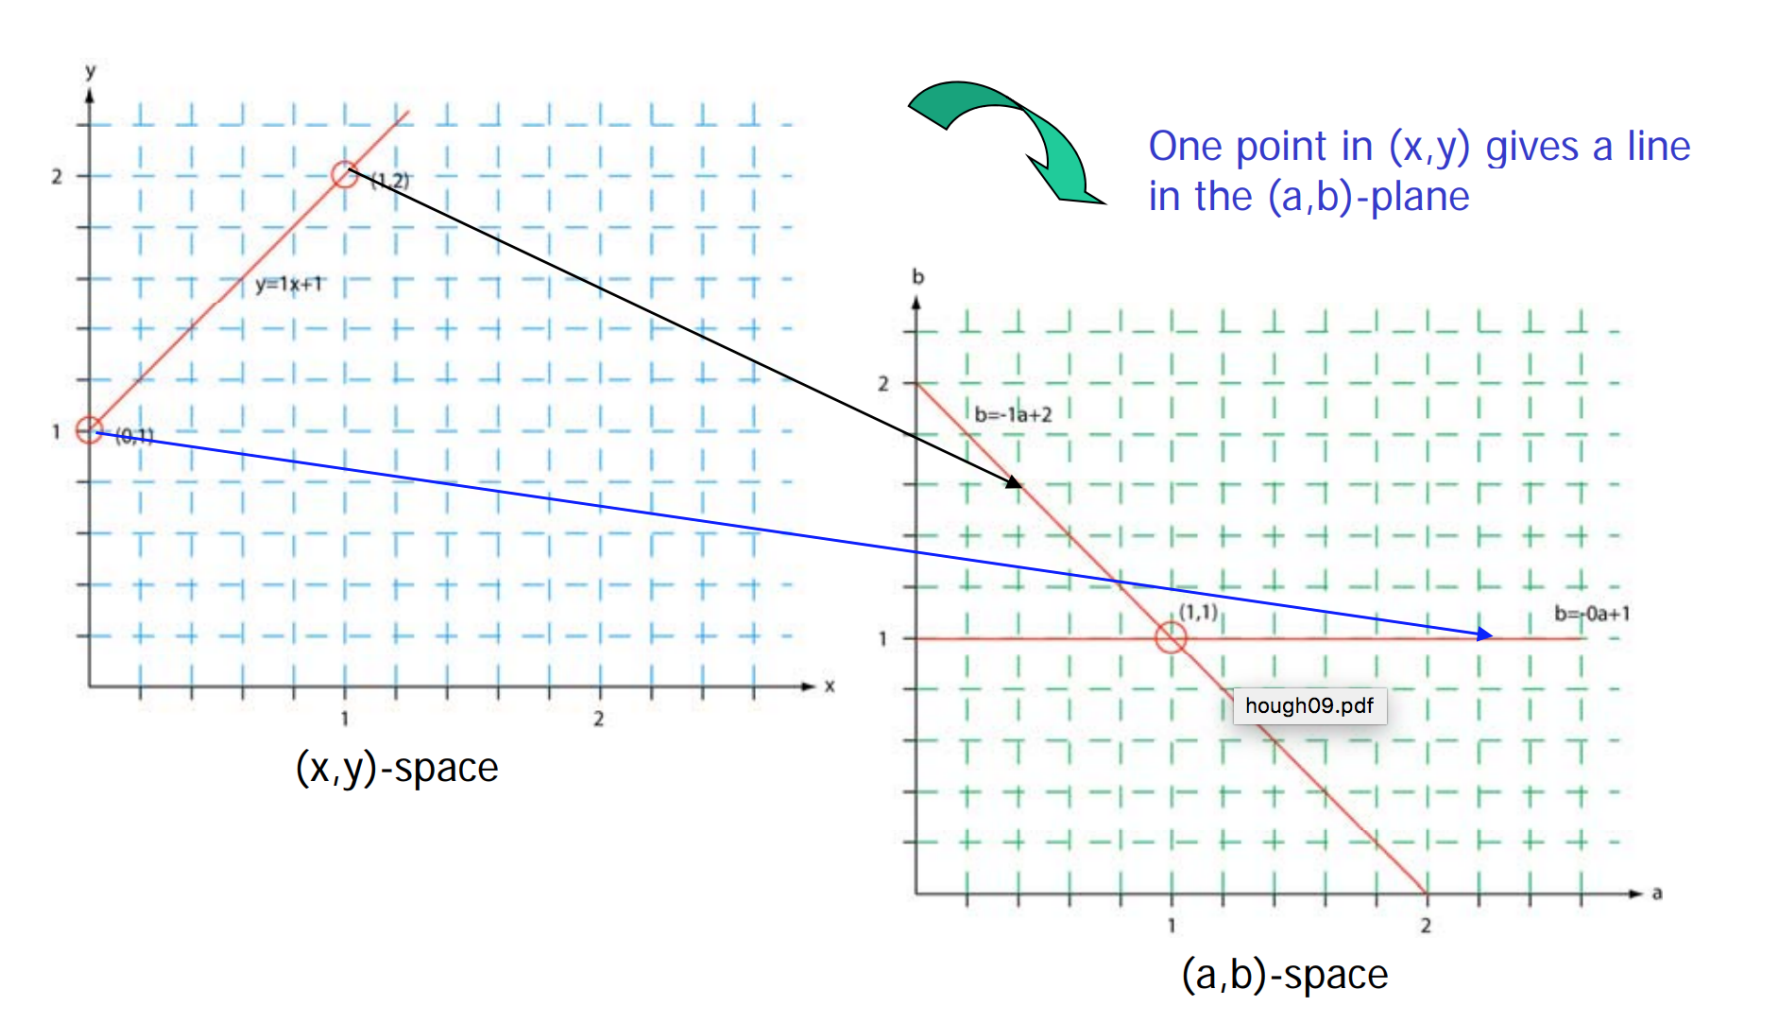
\includegraphics[width=\textwidth]{hough_transform.png}
\textbf{Fig. 3. The transformation from the original space to the Hough space; source: lecture slides}

The intersection of lines in $a,b$ space represent the $a,b$ values that compromise a line $y_i = a*x_i + b$ passing through those points. Example:
Say we have two points $x_1,y_1$ = $(1,1)$, and $x_2,y_2$ = $(2,3)$.
We transform these points into $a,b$ space with the lines $b = -a*1 + 1$ and $b = -a*2 + 3$.
Solving for the intersection of these two lines gives us $a=2$ and $b=-1$. This intersection point in $(a,b)$ space gives us the values for the line that goes through both points in $x,y$ space.

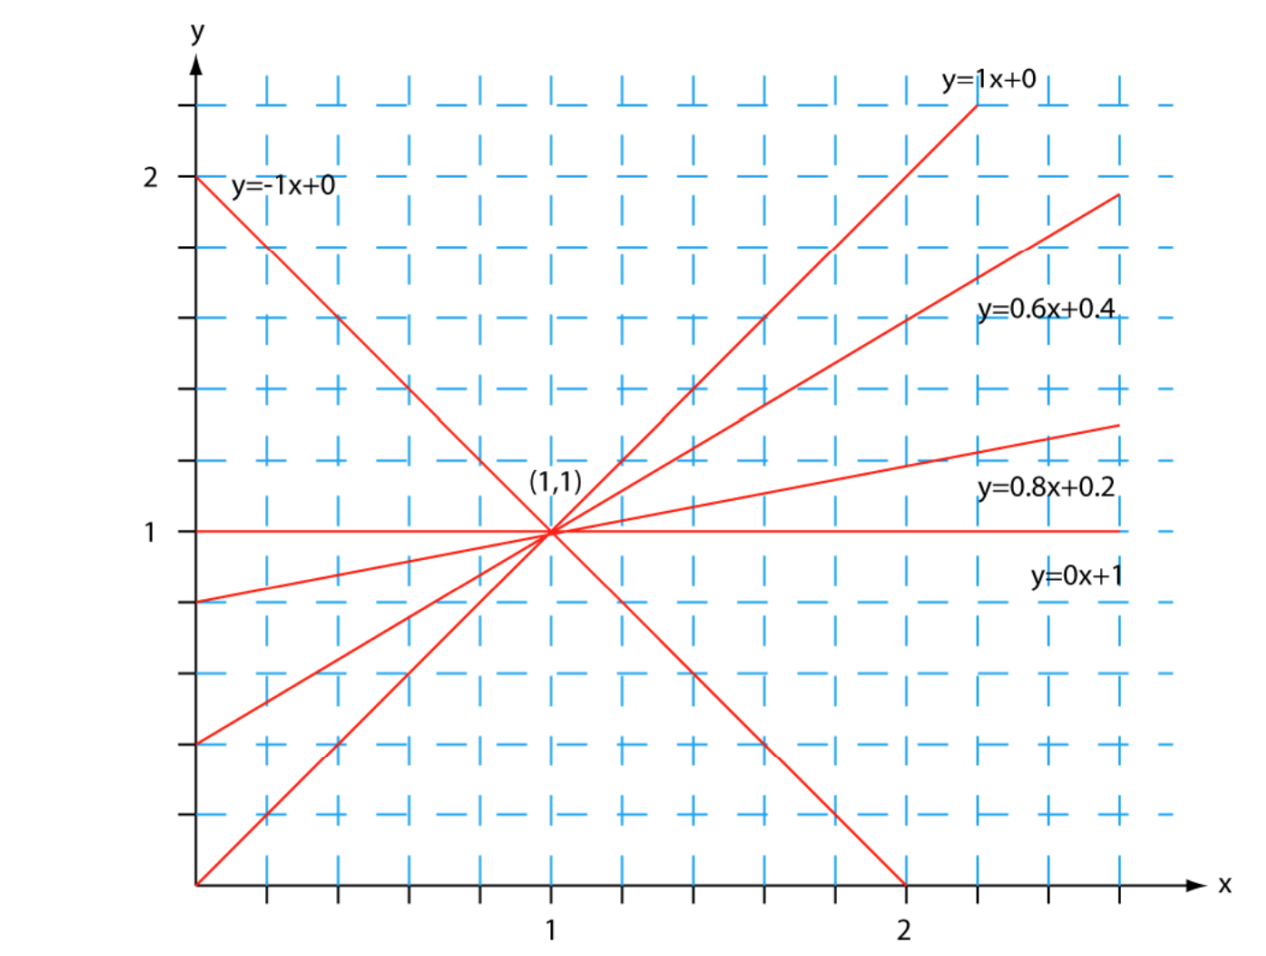
\includegraphics[width=\textwidth]{hough_transform2.png}
\textbf{Fig. 4. The lines passing through a point in the original space; source: lecture slides}

\subsection{Accumulator Cells}
In order to get the "best" lines, we quantize the $a,b$ space into cells. For each line in our $a,b$ space, we add a "vote" or a count to each cell that it passes through. We do this for each line, so at the end, the cells with the most "votes" have the most intersections and therefore should correspond to real lines in our image.

The algorithm for Hough transform in $a,b$ space is as follows:

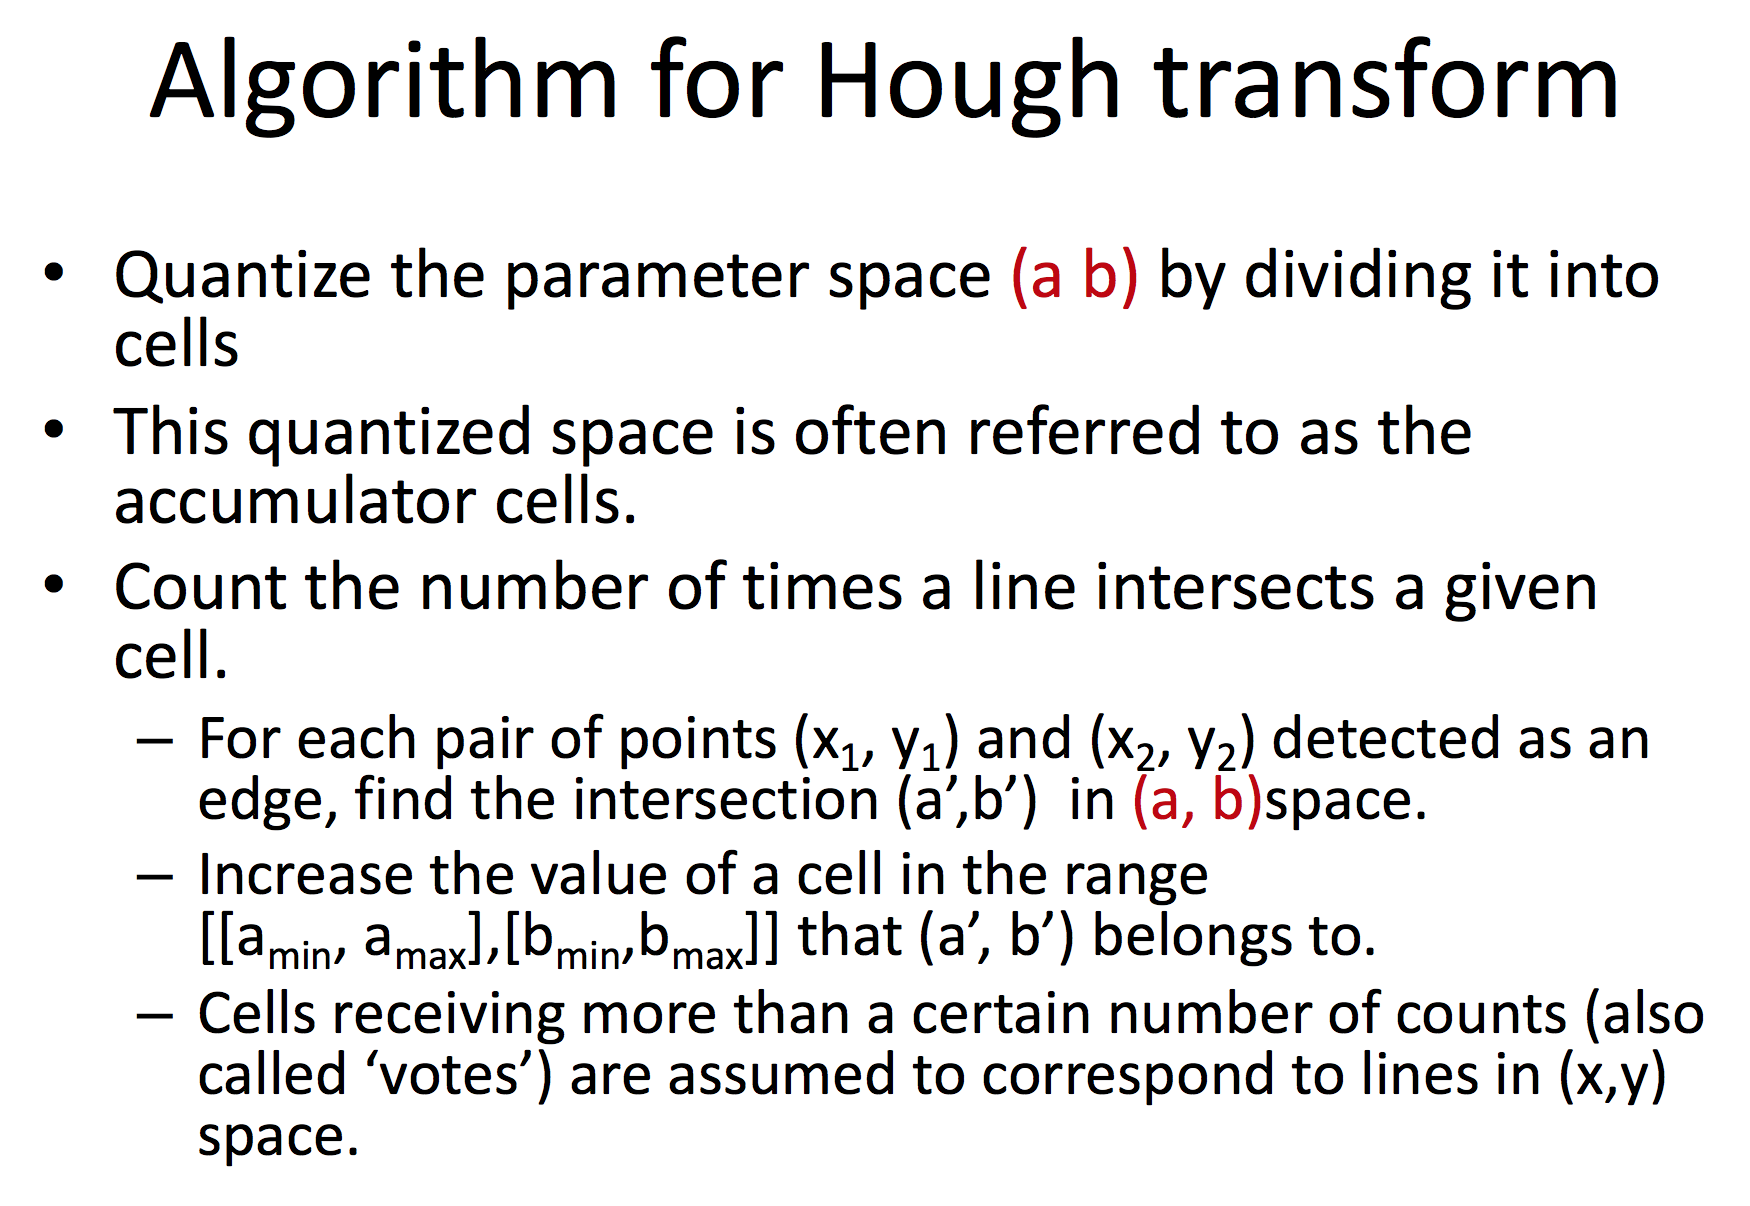
\includegraphics[width=\textwidth]{hough_transform3.png}
\textbf{Fig. 5. The Hough transform algorithm; source: lecture slides}

\subsection{Hough transform in $\rho, \theta$ space}
A problem with using $a,b$ space to represent lines is that they are limited and cannot represent vertical lines.
To solve this, we use polar coordinates to represent lines. For a pixel $x_i, y_i$, we transform it using the equation:
$$ x*\cos\theta + y*\sin\theta = \rho$$
In $\rho, \theta$ space, points are not represented as lines but instead as sine wave-like functions.

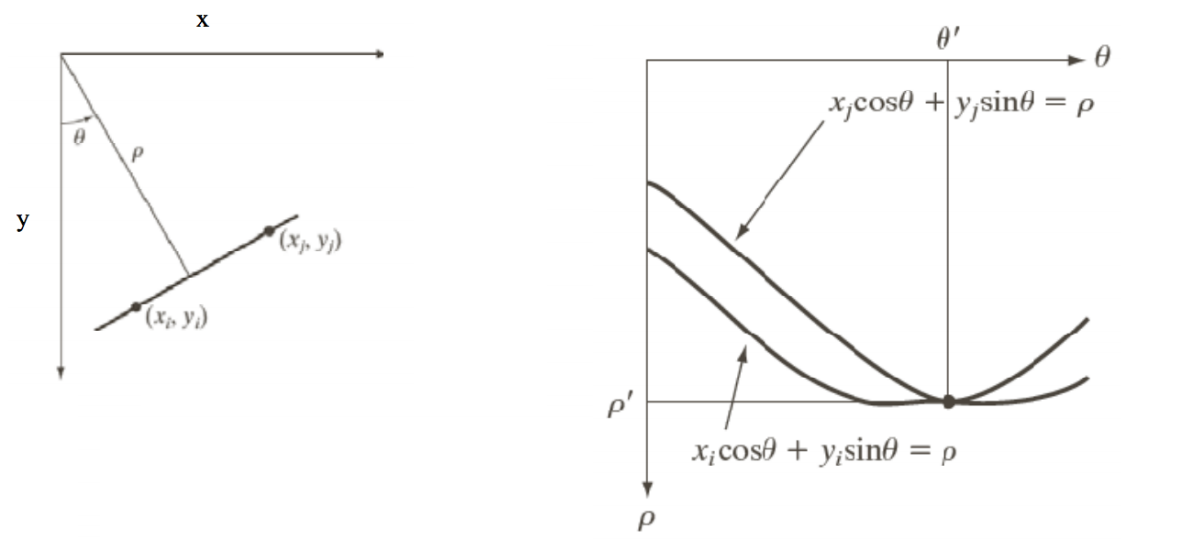
\includegraphics[width=\textwidth]{hough_transform4.png}
\textbf{Fig. 6. The Hough transform in $\rho, \theta$ space; source: lecture slides}

The intersection of these functions in $\rho, \theta$ space still correspond to the $\rho, \theta$ that comprise a line passing through those points.

So, for each pixel $x_i, y_i$ we transform it into a function in  $\rho, \theta$ space. We apply the same accumulator cell algorithm to count the most intersections of functions.

In this case, we quantize our $\rho, \theta$ space into cells, and add a "vote" to each cell that our function passes through. The cells with the most votes are the most likely real lines in our image.

\subsection{Concluding Remarks}
Advantages of the Hough Transform is that it is conceptually simple (just transforming and finding intersection in Hough space). It is also fairly easy to implement, and it can handle missing and occluded data well. Another advantage is that it can find other structures other than lines, as long as the structure has a parametric equation.

Some disadvantages include that it gets more computationally complex the more parameters you have. It can also only look for one kind of structure (so not lines and circles together). The length and the position of a line segment can also not be detected by this. It can be fooled by "apparent" lines, and co-linear line segments cannot be separated.
\section{RANSAC}
With the increase in model complexity (i.e., the number of parameters), the Hough transform loses its effectiveness; this section elaborates on the design of the RAndom Sample Consensus (RANSAC) technique \cite{fischler1981random} which provides a computationally efficient means of fitting models in images. We begin with an introduction of the RANSAC's basic idea and then introduce its algorithm.
\subsection{Introduction to RANSAC Basics}
The RANSAC algorithm is used for estimating the parameters of models in images (i.e., model fitting). The basic idea behind RANSAC is to solve the fitting problem many times using randomly selected minimal subsets of the data and choosing the best performing fit. To achieve this, RANSAC tries to iteratively identify the data points that correspond to model we are trying to fit.

Fig. 7a illustrates an example where a linear model (i.e., 2 parameters) is to be fitted to the data; while the majority of data points fit a linear model, the two points in the top right corner can significantly affect the accuracy of overall fit (if they are included in the fit). The RANSAC algorithm aims to address this challenge by identifying the "inliers" and "outliers" in the data.

RANSAC randomly selects samples of the data, with the assumption that if enough samples are chosen, there will be a low probability that at all samples provides a bad fit.

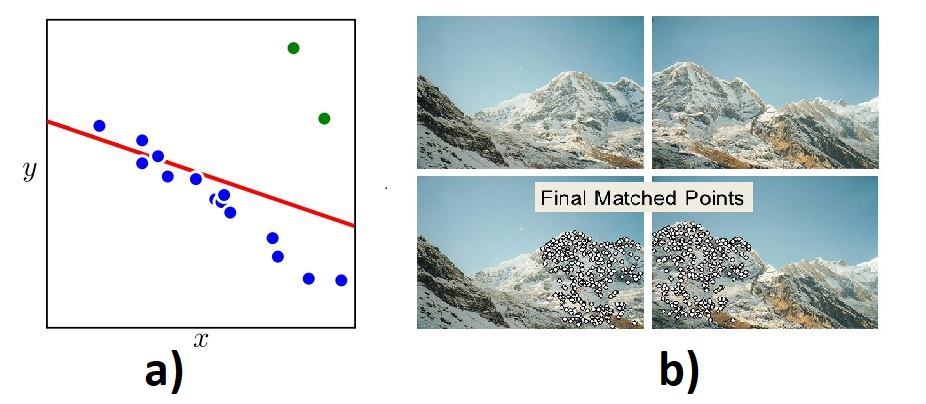
\includegraphics[width=\textwidth]{ransac1.png}
\textbf{Fig. 7. a) the outliers are detected by RANSAC to improve parameter estimation; b) RANSAC application for image stitching; sources(\cite{prince2012computer}and Derek Hoiem)}

\subsection{Applications}
The RANSAC algorithm can be used to estimate parameters of different models; this is proven beneficial in image stitching (Fig. 6b), outlier detection, lane detection (linear model estimation), and stereo camera calculations.

\subsection{The Algorithm}
The RANSAC algorithm iteratively samples nominal subsets of the original data (e.g., 2 points for line estimation); the model is fitted to each sample, and the number of "inliers" corresponding to this fit is calculated; this includes the data points that are close to the fitted model. The points closer than a threshold (e.g., 2 standard deviation, or a pre-determined number of pixels) are considered "inliers". The fitted model is considered good if a big fraction of the data is considered as "inliers" for that fit. In the case of a good fit, the model is re-fitted using all the inliers, and the outliers are discarded. This process is repeated, and model estimates with a big enough fraction of inliers (e.g., bigger than a pre-specified threshold) are compared to choose the best-performing fit. Fig. 8 illustrates this process for a linear model and its three samples. The third sample (Fig. 8c) provides the best fit as it includes the most number of inliers.

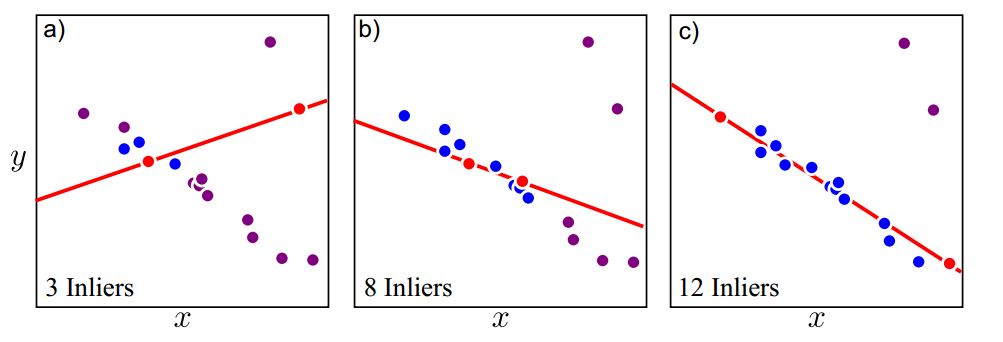
\includegraphics[width=\textwidth]{ransac2.png}
\textbf{Fig. 8. The demonstration of the RANSAC algorithm for a linear model estimation and three random samples; source(\cite{prince2012computer})}


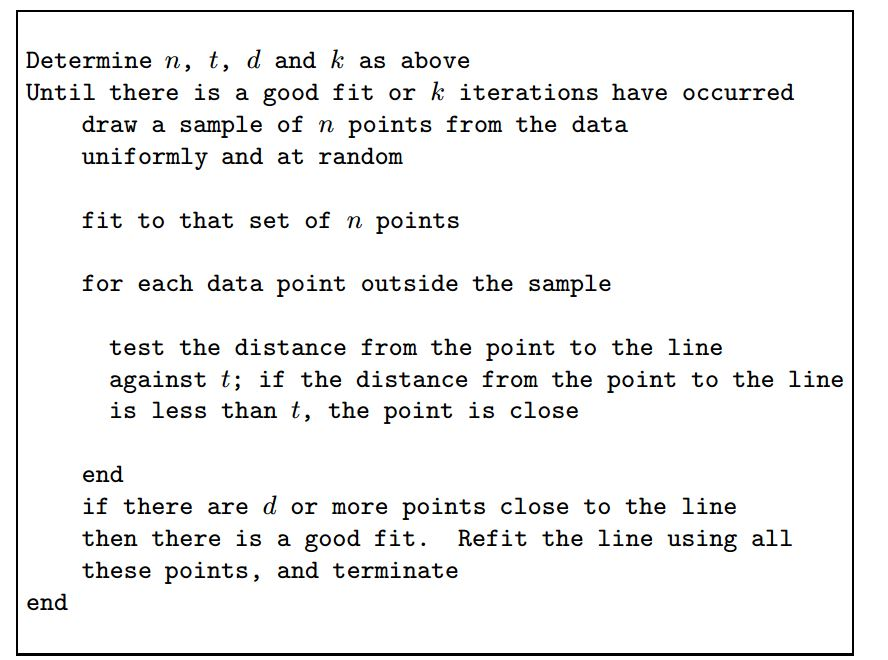
\includegraphics[width=0.9\textwidth]{ransac3.png}

\textbf{Fig. 9. The pseudocode for RANSAC; source(\cite{forsyth2011computer})}

The RANSAC is detailed in Fig. 9. The major steps included in the RANSAC loop:

\begin{enumerate}
  \item Randomly select a seed group from data.
  \item Perform parameter estimation using the selected seed group.
  \item Identify the inliers (points close to the estimated model).
  \item (If there exists a sufficiently large number of inliers,)re-estimate the model using all inliers.
  \item repeat steps 1-4 and finally keep the estimate with most inliers and best fit.
\end{enumerate}

\subsection{How Many Samples are Needed?}
The RANSAC is a non-deterministic model fitting approach; this means that the number of samples need to be large enough to provide a high confidence estimate of parameters. The number of required samples depends on 1) the number of fitted parameters and 2) the amount of noise. Fig. 10 lists the minimum number of samples needed based on p=0.99 and variations of sample size (i.e., the number of parameters) and the fraction of outliers (i.e., noise). More samples are needed for estimating bigger models and noisier data.
A large enough number of samples ($k$) need to be chosen such that a low probability of only seeing bad samples (${P_f}$) is guaranteed:
$${P_f}= (1-W^n)^k= 1-p$$
where $W$ and $n$ are respectively the fraction of inliers and the number of points needed for model fitting. The minimum number of samples:
$$k=\frac{log(1-p)}{log(1-W^n)}$$

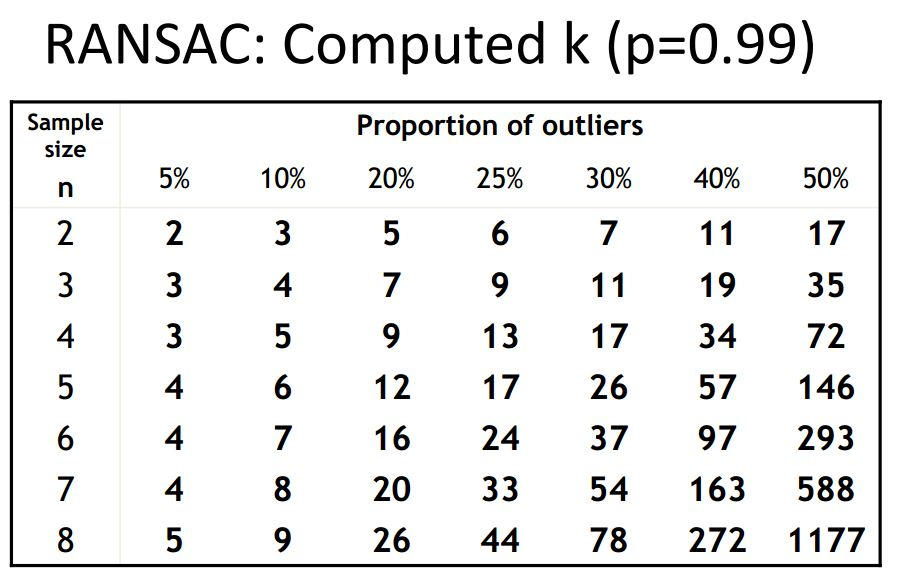
\includegraphics[width=\textwidth]{ransac4.png}
\textbf{Fig. 10. The number of samples for different choices of noise population and model size; source: David Lowe)}

\subsection{Advantages, Limitations, and Considerations}
The advantages of the RANSAC lie in its simple implementation and wide application range in the model fitting domain. Other advantages include its computational efficiency; the sampling approach provides a better alternative to solving the problem for all possible combinations of features.

In some cases, it'd be more efficient to use the Hough transform instead of the RANSAC:
\begin{enumerate}
  \item The number of parameters are small; for example, linear model estimation (2 parameters) can be achieved efficiently using Hough transform, while image stitching requires a more computationally frugal approach such as RANSAC.
  \item If the noise population is high; as we saw earlier, increase in noise requires a more extensive sampling approach (higher number of samples), increasing computation cost. Increased noise reduces the chances of correct parameter estimation and the accuracy of inlier classification.
\end{enumerate}

The poor performance in highly noisy data is a primary limitation of the RANSAC; this is espcially crucial as real-world problems have high rate of outliers.

% References
\small
\bibliographystyle{plain}
\bibliography{bibliography}


\end{document}
